\setchapterpreamble[u]{\margintoc}
\chapter{单因素实验设计}
\labch{options}

\subsection{良好实验在统计上的体现}
以往在论述实验设计时,我们称随机区组设计和被试内可以带走使实验更加数来宝这样一个事实,但这只是描述性的话,没有数据的前后对比无法让人真的信服随机区组和被试内设计的好处.所以,现在要从数据上看到$F$怎样更容易显著.

所谓$F$更容易显著无非就是$F$更大了($F=MSA/MSE$),想让$F$变大有两个手段,让处理效应($MSA$)变大,或者让误差效应($MSE$)变小,这件事情在前面已经介绍过.我说过心理学家感兴趣的那些现象往往都不太大\sidenote{也可以说是效应量(effect size)总是不太大},而且人为加大处理效应有时没有什么意义.从实验设计的角度上,减小误差才是关键.

\begin{marginfigure}
	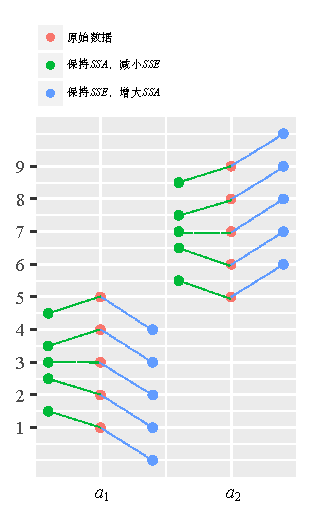
\includegraphics{SSA_SSE}
	\caption{红色是原始数据,蓝色代表组内误差不变,加大处理效应;绿色代表组间变异不变,改变组内误差}
	\labfig{SSA_SSE}
\end{marginfigure}

这就好比用天文望远镜观测外太空,我想发现人们不曾发现过的行星,我透过天文望远镜可以看到一些噪音——没有规律发亮的光点,但是那颗星星好像也在发光,我想鉴别这个星星是否真实存在,但是这件事情不是那么容易,因为星星发的光和噪音总是同时出现,故只有星星发出的光足够大,大到和周围的噪音是那么的与众不同,我再将这个星星是噪音有很大几率犯错,我才敢认定那是星星.我们清楚地知道,想要更加清楚地观察到星星无非有两种手段,其一是让星星在原有基础上多发电光;其二是让周围的噪音降低点.

方差分析模型中的$MSA$和$MSE$是相互独立的,它们俩可以独立地变化.随机误差指的是由随机因素导致数据在理想值周围随机晃动的偏差,它要是和处理不独立那就不能叫随机误差了.

\begin{kaobox}[frametitle=思考]
假定我们有一组分数,分别计算出$MSA$和$MSE$.\\
(1)我们可以改变$AS$\sidenote[*5][]{$AS$中A代表因素$A$的处理效应,$S$代表被试个体误差,具体是什么后面再说}分数,保持处理平均数恒定.即保持$MSA$不变而改变$MSE$.\\
(2)如果我们改变组平均数,处理组内分数关系不就,$MSA$会变化,而$MSE$不就.表明两个均方是独立变化的.



\end{kaobox}

我们看一组数据
\begin{align*}
    a_1:1, 2, 3, 4, 5\\
    a_2:5, 6, 7, 8, 9
\end{align*}

(1)调整原始数据,保持$SSA$不变,而$SSE$改变(减小$SSE$) (通常加大处理效应实现)

(2)调整原始数据,改变$SSA$不变(增大$SSA$),而$SSE$不变

我直接给出我的思路,\reffig{SSA_SSE}中红色是原始数据,它有两个水平,$a_1$的各个值围绕其均值3波动,$a_2$的各个值围绕其均值7波动.

绿色是我写的符合(1)的一组数据,可以看到红色数据$a_1$处理的每个数据都围绕着3波动,现在绿色的值在$a_1$内还是围绕3波动,但是数据间的距离更短了,它们显得更加紧密.虽然从组内均值上来看(3和7)两组数据的平均值之差不变,但是由于$a_1$的数据更集中于3,$a_2$的数据更集中于7,故实际上这样两组间的差异其实增大了.

蓝色是我写的符合(2)的一组数据,可以看到数据间的紧密程度不变,$a_1$整体向下移动,$a_2$整体向上移动,这样组间的差距被拉大.

原始数据方差分析结果是.

\begin{table}[h]
	\centering
	\caption{原始数据方差分析}
	\labtab{RAW_ANOVA}
	{
		\begin{tabular}{cccccc}
			\toprule
			变异来源 & $SS$ & $df$ & $MS$ & $F$ & $p$  \\
			\midrule
			组间变异 & 40.000 & 1.000 & 40.000 & 16.000 & 0.004  \\
			组内变异 & 20.000 & 8.000 & 2.500 &  &    \\
			\bottomrule
			% \addlinespace[1ex]
			% \multicolumn{6}{p{0.5\linewidth}}{\textit{Note.} Type I Sum of Squares} \\
		\end{tabular}
	}
\end{table}

\begin{margintable}
    \caption{保持$SSA$不变,减小$SSE$}
    \labtab{lower_SSE}
    \raggedright
    \begin{tabular}{cccccc}
        \hline
        $a_1$ & 1.5 & 2.5 & 3 & 3.5 & 4.5\\
        $a_2$ & 5.5 & 6.5 & 7 & 7.5 & 8.5\\
        \hline
    \end{tabular}
\end{margintable}

绿色数据见\vreftab{lower_SSE}.


其方差分析结果是,可以看到相比\vreftab{RAW_ANOVA}中的数据,处理效应没变,误差效应减小了,$F$值变大,$p$值减小.

\begin{table}[h]
	\centering
	\caption{绿色数据方差分析}
	\label{tab:aNOVA-Score}
	{
		\begin{tabular}{cccccc}
			\toprule
			变异来源 & $SS$ & $df$ & $MS$ & $F$ & $p$  \\
			\midrule
			组间变异 & 40.000 & 1.000 & 40.000 & 32.000 & $<$ .001  \\
			组内变异 & 10.000 & 8.000 & 1.250 &  &    \\
			\bottomrule
			% \addlinespace[1ex]
			% \multicolumn{6}{p{0.5\linewidth}}{\textit{Note.} Type III Sum of Squares} \\
		\end{tabular}
	}
\end{table}

\begin{margintable}
    \caption{保持$SSE$不变,增大$SSA$}
    \labtab{UPPER_SSA}
    \raggedright
    \begin{tabular}{cccccc}
        \hline
        $a_1$ & 1 & 1 & 2 & 3 & 4\\
        $a_2$ & 6 & 7 & 8 & 8 & 10\\
        \hline
    \end{tabular}
\end{margintable}

蓝色数据见\vreftab{UPPER_SSA}.

其方差分析结果是,可以看到相比\vreftab{RAW_ANOVA}中的数据,处理效应变大,组内误差减没变,$F$值变大,$p$值减小.

\begin{table}[h]
	\centering
	\caption{蓝色数据方差分析}
	\label{tab:aNOVA-Score}
	{
		\begin{tabular}{cccccc}
			\toprule
			变异来源 & $SS$ & $df$ & $MS$ & $F$ & $p$  \\
			\midrule
			组间变异 & 90.000 & 1.000 & 90.000 & 36.000 & $<$ .001  \\
			组内变异 & 20.000 & 8.000 & 2.500 &  &    \\
			\bottomrule
			% \addlinespace[1ex]
			% \multicolumn{6}{p{0.5\linewidth}}{\textit{Note.} Type III Sum of Squares} \\
		\end{tabular}
	}
\end{table}




\section{单因素完全随机实验设计}
\subsection{基本特点}

完全随机设计(completely randomized design)的假定是,由于被试是从总体中随机选取,处理也是随机分配给被试,那么被试间的差异也是随机、在统计上无差异的.

\begin{margintable}
	\centering
	\caption{单因素完全随机实验设计中被试的分配}
	\labtab{one_way_ANOVA_data}
	{
		\begin{tabular}{cccc}
			\toprule
			$a_1$ & $a_2$ & $a_3$ & $a_4$ \\
			\midrule
			$S_1$ & $S_2$ & $S_3$ & $S_4$ \\
			$S_5$ & $S_6$ & $S_7$ & $S_8$ \\
			$S_9$ & $S_{10}$ & $S_{11}$ & $S_{12}$ \\
			$S_{13}$ & $S_{14}$ & $S_{15}$ & $S_{16}$ \\
			\bottomrule
			% \addlinespace[1ex]
			% \multicolumn{6}{p{0.5\linewidth}}{\textit{Note.} Type III Sum of Squares} \\
		\end{tabular}
	}
\end{margintable}

单因素完全随机设计中分配被试的图解例子如\vreftab{one_way_ANOVA_data},
个因素$A$有4个水平,每个处理下有4个被试.完全随机设计是一种被试间设计,这意味着每一个被试只接受一种处理或处理的组合
\sidenote[*-5][]{处理的组合是多因素实验中会遇到的,后面遇到了再说}
,故对于本例而言需要16个被试.

对按下来要描述的模型的字母进行一下简要的说明:

(1)假设因素$A$有$p$个水平,用$\alpha _j$表示其第$j$个水平($1 \leq j \leq p$),也就是说$A$的水平分别是$\alpha _1,\cdots,\alpha _j,\cdots, \alpha _p$,

(2)$p$个处理下的被试数都相等,均为$n$个,用$i$表示每个处理下第$i$个被试($1 \leq i \leq n$)

(3)假设被试在没有施加处理的时候,无限次实验结果的平均数是$\mu$.该值是个理想值,其实意思是被试测量值在理论上的基线,不过这么说只是表达了概念.虽然说明了更加明确的定义不过可以充分的感受到,这个理论基线值是无法获得的,毕竟无限次是个极限,不是一个具体的数,所以$\mu$是个理论值.

(4)假设实验中的误差是$\varepsilon _{i\left(j\right)}$
\sidenote{关于为什么它的下标是带括号的现在不便解释.}
,其平均数为0,方差为$\sigma _e^2$,我们进一步假设它服从正态分布

(4)观察值$Y_{ij}$指第$j$个处理水平下,第$i$个被试的观测值

后现的章节因素多了会加入一些新字母和下标,和上述符号已经没有本质区别,故以后我不打算再介绍新符号了.

单因素完全随机设计的原假说是:多个处理水平上的总体平均数相等,即
$$
H_0: \mu _{.1}=\mu _{.2}=\cdots=\mu _{.p}
$$

或处理效应等于为0,即
$$
\alpha _j=0
$$


单因素完全随机实验设计模型
\begin{equation}
    Y_{ij}=\mu +\alpha _j+\varepsilon _{i\left( j \right)}
\end{equation}

其中:

\begin{tabular}{lcl}
    $Y_{ij}$ & - & 被试$i$在处理水平$j$上的分数 \\
    $\mu$ & - & 总体平均数 \\
    $\alpha _j$ & - & 水平$j$的处理效应 \\
    $\varepsilon_{i \left( j \right)}$ & - & 误差效应 \\
\end{tabular}



\subsection{实验设计与计算举例}

\subsubsection{研究的问题}
我想研究文章的生字密度对学生阅读理解的影响.我的假设是:阅读理解随着文章中生字密度的增加而下降。因此,该实验有一个自变量——生字密度,通过研究前人文献我感兴趣的是四种生字密度
(1)$5:1\left(a_1\right)$、
(2)$10:1\left(a_2\right)$、
(3)$15:1\left(a_3\right)$、
(4)$20:1\left(a_4\right)$
因变量是被试的阅读理解分数。实施实验时,我将32名被试随机分成四组,每组被试阅读一种生字密度的文章,并回答阅读理解测验中有关文章内容的问题。这是一个典型的单因素完全随机设计。虽然我不再检验实验中其他因素的影响,但实际上存在着诸多对因变量影响的无关变量,比如文章的长度、文章的主题熟悉性、文章类型等,还有被试的年龄、受教育程度、阅读能力等。这时,控制无关变量可做的工作之一是在选取四篇文章时,使它们在除生字密度以外的其他方面尽量匹配。

\subsubsection{新的计算模型的引入以及数据的计算}
我将引入一种新的计算模式,这种模式主要是为了手算.为了理解愿意,我们必须手算一次每种实验设计的简单数据,但是用统计教材上的算法根本无法实现一个较为精确的估算,其原因是,和方的计算公式选用:

$$
    SS =
        \sum\limits_{i=1}^{n}
        \left( 
            X_i -\bar{X} 
        \right)^2
$$

式子中$\bar{X}$很大可能是小数,且可能是循环小数,所以每次相减都会四舍五入,然后平方后进一步放大误差,这样算到最后误差不断累记.所以应当最后一步再做除法,把上面的式子改写一下:

\begin{align*}
SS= & \sum\limits_{i=1}^n{\left( X_i-\bar{X} \right) ^2}
\\
    & =\sum\limits_{i=1}^n{\left( X_{i}^{2}+\underset{\text{常数}}{\underbrace{\bar{X}^2}}-\underset{\text{常数}}{\underbrace{2\bar{X}}}X_i \right)}
\\
    & =\sum\limits_{i=1}^n{X_{i}^{2}}+n\bar{X}^2-\underset{2n\bar{X}^2}{\underbrace{2\bar{X}\sum\limits_{i=1}^n{X_i}}}
\\
    & =\sum\limits_{i=1}^n{X_{i}^{2}}-n\left( \frac{\sum\limits_{i=1}^n{X_i}}{n} \right) ^2
\\
    &= \underset{\text{离散+集中+可能个体差异}}{\underbrace{\sum\limits_{i=1}^n{X_{i}^{2}}}}-\underset{\text{集中}}{\underbrace{\frac{\left( \sum\limits_{i=1}^n{X_i} \right) ^2}{n}}}
\end{align*}

这样除法只进行了一次(上式“集中”那里算了一次除法,产生误差),其余的都是乘法和加法.那么在方差分析中,大量求$SS$,用这样的方法就可以利于手算,以便更好了解方差分析原理.


\textbf{1.计算表}

\begin{margintable}
	\centering
	\caption{单因素完全随机实验的$AS$表}
	\labtab{one_way_ANOVA_AS_TAB}
	{
		\begin{tabular}{cccccc}
			\toprule
    			     & $a_1$ &  $a_2$ &  $a_3$ &  $a_4$ & \\
    			     \midrule
                              & \cellcolor[rgb]{ .949,  .949,  .949}3 & \cellcolor[rgb]{ .949,  .949,  .949}4 & \cellcolor[rgb]{ .949,  .949,  .949}8 & \cellcolor[rgb]{ .949,  .949,  .949}9 &  \\
                              & \cellcolor[rgb]{ .949,  .949,  .949}6 & \cellcolor[rgb]{ .949,  .949,  .949}6 & \cellcolor[rgb]{ .949,  .949,  .949}9 & \cellcolor[rgb]{ .949,  .949,  .949}8 &  \\
                              & \cellcolor[rgb]{ .949,  .949,  .949}4 & \cellcolor[rgb]{ .949,  .949,  .949}4 & \cellcolor[rgb]{ .949,  .949,  .949}8 & \cellcolor[rgb]{ .949,  .949,  .949}8 &  \\
                              & \cellcolor[rgb]{ .949,  .949,  .949}3 & \cellcolor[rgb]{ .949,  .949,  .949}2 & \cellcolor[rgb]{ .949,  .949,  .949}7 & \cellcolor[rgb]{ .949,  .949,  .949}7 &  \\
                              & \cellcolor[rgb]{ .949,  .949,  .949}5 & \cellcolor[rgb]{ .949,  .949,  .949}4 & \cellcolor[rgb]{ .949,  .949,  .949}5 & \cellcolor[rgb]{ .949,  .949,  .949}12 &  \\
                              & \cellcolor[rgb]{ .949,  .949,  .949}7 & \cellcolor[rgb]{ .949,  .949,  .949}5 & \cellcolor[rgb]{ .949,  .949,  .949}6 & \cellcolor[rgb]{ .949,  .949,  .949}13 &  \\
                              & \cellcolor[rgb]{ .949,  .949,  .949}5 & \cellcolor[rgb]{ .949,  .949,  .949}3 & \cellcolor[rgb]{ .949,  .949,  .949}7 & \cellcolor[rgb]{ .949,  .949,  .949}12 &  \\
                              & \cellcolor[rgb]{ .949,  .949,  .949}2 & \cellcolor[rgb]{ .949,  .949,  .949}3 & \cellcolor[rgb]{ .949,  .949,  .949}6 & \cellcolor[rgb]{ .949,  .949,  .949}11 &  \\
                              \midrule
                        总     & \cellcolor[rgb]{ .886,  .937,  .855}35 & \cellcolor[rgb]{ .886,  .937,  .855}31 & \cellcolor[rgb]{ .886,  .937,  .855}56 & \cellcolor[rgb]{ .886,  .937,  .855}80 & \cellcolor[rgb]{ .867,  .922,  .969}202 \\
			\bottomrule
		\end{tabular}
	}
\end{margintable}

\vreftab{one_way_ANOVA_AS_TAB}中的数据被我标了3个颜色,不同颜色的区域反映了不同的变异,一个一个来看.灰色数据可以看到集中趋势、离散趋势,包含个体差异;绿色数据看不到个体差异,但是能看到组间差异;蓝色数据只能看到集中趋势.

某个区域的颜色为$L$,定义这个区域反应的变异$[\text{因素}]$的算法:

\[
\left[ A?B?C?\cdots S? \right] =\frac{\sum{\left( \text{某颜色区域的数据}^2 \right)}}{\text{该颜色一个单元格内被试数}}
\]

公式中的$?$表示的是前面的因素可有可无.如果你感觉有些抽象,不妨直接看一下下面是在单因素完全随机实验设计中是怎么计算的.
以后所有的$SS$都是这样的算法.列表算$SS$的好处在多因素实验设计中会充分展现,现在可能还是显得麻烦.

\textbf{2.各种基本量的计算}
    \[
        \sum\limits_{i=1}^{n} \sum\limits_{j=1}^{p}Y_{ij} = 3+6+4+\cdots=202.000\\
    \]
    \begin{align*}
        %----------------------------------------------------------
        %[Y]
            \frac{
                \left(
        	\sum\limits_{i=1}^{n} \sum\limits_{j=1}^{p}Y_{ij}
                \right)^2}
            {np}=& \colorbox[rgb]{ .867,  .922,  .969}{$[Y]$} = 
            \frac{
                \left(
        	    202
                \right)^2}
                {
                    \left(
        	           8
                    \right)^2
                    \left(
                        4
                    \right)^2
                }&=1275.125\\
        %----------------------------------------------------------
        %[AS]
            \sum\limits_{i=1}^{n} \sum\limits_{j=1}^{p}Y_{ij}^2=
            & \colorbox[rgb]{ .949,  .949,  .949}{$[AS]$} = 
            \left(
            	3
            \right)^2 +
            \left(
            	6
            \right)^2    +\cdots &=1544.000\\
        %----------------------------------------------------------
        %[A]    
            \sum\limits_{i=1}^{n}
            \frac
                {\left(
	            \sum\limits_{j=1}^{p}Y_{ij}
                \right)^2}
                {n}=
            &\colorbox[rgb]{ .886,  .937,  .855}{$[A]$}=
            \frac{\left(35\right)^2}{8}+\frac{\left(31\right)^2}{8}+\cdots&=1465.250            
    \end{align*}

其中,$[Y]$仅仅用了右下角的数据,这里的数据只有集中趋势,不体现个体差异,也不体现离散趋势,用字母$Y$表示集中趋势;$[A]$用到了下方绿色的数据,这部分数据由于合并了组内的数据,所以不体现个体差异,不过还能体现离散趋势和集中趋势.用字母$A$表示因素$A$的集中和离散趋势,要得到纯粹的$A$的离散趋势还要减去$[Y]$这个集中趋势;$[AS]$用到了中间灰色区域的数据,体现了集中趋势,也体现了离散趋势,而且每个个体的数据都用到了,故也能体现个体差异,$[AS]$中各个符号前面都出现过,其中$A$代表了因素$A$的集中和离散趋势,$S$表示是个体差异.

由上面的分析可以看出,只有原始数据可以反映个体差异$S$,只要合并了数据就损失了个体差异;
离散趋势只要有多组数据都可以反映;
所有的数据都一定会反映集中趋势,故在所有式子都不再加入$Y$,否则过于麻烦.

\textbf{3.平方和分解与计算}
\begin{alignat*}{3}
& SS_{\text{总}}       && = SS_{\text{组间}}+SS_{\text{组内}}\\
& SS_{\text{总}}       && = [AS]-[Y]        &&  =268.875\\
& SS_{\text{组间}}     && = SSA=[A]-[Y]     &&  =190.125\\
& SS_{\text{组内}}     && = SSE=SS_{\text{总}}-SS_{\text{组间}}  && =78.750
\end{alignat*}

\textbf{4.方差分析表及结果的解释}

\begin{table}[h]
	\centering
	\caption{单因素完全随机设计的方差分析表}
	\labtab{one_way_ANOVA_Tab}
	{
		\begin{tabular}{lrrcrrr}
			\toprule
			\multicolumn{1}{c}{变异源} & \multicolumn{1}{c}{$SS$} & \multicolumn{1}{c}{$df$} & \multicolumn{1}{c}{$MS$} & \multicolumn{1}{c}{$F$} & \multicolumn{1}{c}{$p$} \\
			\midrule
			组间(生字密度) & 190.125 & $p-1=3$ & 63.375 & 22.533 & $<$ .001  \\
			组内(个体误差) & 78.750 & $p(n-1)=28$ & 2.813 &  &    \\
			\midrule
			总计 & 268.875 & $np-1=31$ & & &\\
			\bottomrule
			% \addlinespace[1ex]
			% \multicolumn{6}{p{0.5\linewidth}}{\textit{Note.} Type III Sum of Squares} \\
		\end{tabular}
	}
\end{table}

方差分析结果表明,生字密度的效应是显著的($F(3,28)=22.53(p<0.01)$),生字不同的文章对学生的学生阅读理解有显著的影响。从阅读理解的四种生字密度文章的平均数可以初步看出

\textbf{5.平方和与自由度分解图}
\begin{equation}
    SS_{\text{总}} \begin{cases}
    SS_{\text{组间}}\\
    SS_{\text{组内}}
\end{cases}
\end{equation}
\[
    SS_\text{总} \quad df=np-1=31\\
    SS_{\text{组间}} \quad df=p-1=3\\
    SS_{\text{组内}} \quad df=p(n-1)=28
\]

\subsection{一些解释}

\textbf{1.各种平方和的意义}

\begin{description}
\item[$SS_{\text{总变异}}$] ——总平方和或总变异,带有实验数据中所有的变异,包括实验处理效应、无关变异和误差变异.
\item[$SS_{\text{组间}}$]——组间平方和,或处理平方和,指所有由于实验处理引起的变异,在单因素设计中指$A$因素的处理效应.
\item[$SS_{\text{组内}}$]——组内平方和,或误差平方和,指所有不能用实验处理解释的变异,它可能包括被试个体差异、其他无关变异和实验误差.在单因素完全随机实验中,不再对组内平方和做进一步分离,因此在总变异中减去组间平方和就是组内平方和.
\end{description}

完全随机实验中$F$值的计算是:
\[
F=\frac{MS_{\text{组间}}}{MS_{\text{组内}}}
\]

$F$值的实质是两个卡方商的分布,而$(n-1)S^2/\sigma ^2 \sim \chi ^2_{n-1}$
,故$F$值可以比较两个方差是否存在显著差异,在方差分析中就是检验实验处理带来的效应是否不同于实验误差,如果差异达互一定统计显著水平,表明处理的效应是存在的.

\textbf{2.方差显著的意义}

方差分析显著表明,从整体来看组间的平均数是有差异的,即$\alpha _1 \dots \alpha _p$不完全相等
\sidenote{即:$\exists \,\, 1 \leq u,v \leq p, \alpha _u \neq \alpha _v $}
,但是具体那些存在差异不知道.想检验到底是哪些平均数间存在差异要进行比较和对比,这不是本章的内容,因此不介绍了.

\textbf{3.同质性检查}

\begin{margintable}
	\centering
	\caption{计算单元内误差}
	\labtab{one_way_ANOVA_WITHIN_ERROR}
	{
		\begin{tabular}{cccc}
			\toprule
    			     $a_1$ &  $a_2$ &  $a_3$ &  $a_4$ \\
    			     \midrule
                            \rowcolor[rgb]{ .949,  .949,  .949} 3     & \cellcolor[rgb]{ .867,  .922,  .969}4 & \cellcolor[rgb]{ .886,  .937,  .855}8 & \cellcolor[rgb]{ .988,  .894,  .839}9 \\
                            \rowcolor[rgb]{ .949,  .949,  .949} 6     & \cellcolor[rgb]{ .867,  .922,  .969}6 & \cellcolor[rgb]{ .886,  .937,  .855}9 & \cellcolor[rgb]{ .988,  .894,  .839}8 \\
                            \rowcolor[rgb]{ .949,  .949,  .949} 4     & \cellcolor[rgb]{ .867,  .922,  .969}4 & \cellcolor[rgb]{ .886,  .937,  .855}8 & \cellcolor[rgb]{ .988,  .894,  .839}8 \\
                            \rowcolor[rgb]{ .949,  .949,  .949} 3     & \cellcolor[rgb]{ .867,  .922,  .969}2 & \cellcolor[rgb]{ .886,  .937,  .855}7 & \cellcolor[rgb]{ .988,  .894,  .839}7 \\
                            \rowcolor[rgb]{ .949,  .949,  .949} 5     & \cellcolor[rgb]{ .867,  .922,  .969}4 & \cellcolor[rgb]{ .886,  .937,  .855}5 & \cellcolor[rgb]{ .988,  .894,  .839}12 \\
                            \rowcolor[rgb]{ .949,  .949,  .949} 7     & \cellcolor[rgb]{ .867,  .922,  .969}5 & \cellcolor[rgb]{ .886,  .937,  .855}6 & \cellcolor[rgb]{ .988,  .894,  .839}13 \\
                            \rowcolor[rgb]{ .949,  .949,  .949} 5     & \cellcolor[rgb]{ .867,  .922,  .969}3 & \cellcolor[rgb]{ .886,  .937,  .855}7 & \cellcolor[rgb]{ .988,  .894,  .839}12 \\
                            \rowcolor[rgb]{ .949,  .949,  .949} 2     & \cellcolor[rgb]{ .867,  .922,  .969}3 & \cellcolor[rgb]{ .886,  .937,  .855}6 & \cellcolor[rgb]{ .988,  .894,  .839}11 \\
                            \midrule
                            35 & 31 &  56 & 80\\
                        \bottomrule
		\end{tabular}
	}
\end{margintable}

$F$检验要求被试在观测值上的变异是相同的,这靠随机化完成,检验是否真的做到了同质性就要进行同质性检验.
同质性的要求是处理前被试同质,在心理学实验中通常不进行前测,因为我们假定实验处理不影响随机因素,故处理后处理内被试的差异也反映了处理前被试间的个体差异,比如在\reffig{SSA_SSE}中红色点在不同处理水平的分散水平都一样,$a_1$下它们离各个相近的点相差1,$a_2$下它们还是这样.

严格的因果关系要求让因变量的差异仅由自变量不同水平造成,研究者操纵自变量在不同水平上变化,除了自变量不同之外,其余的变量都是无关变量,需要全部保持恒定.不过这点在以人为研究对象的实验中无法达到,不同人在进入实验室前就已经历了他/她自己独一无二的人生,因此实验即使控制地再严密,接受相同的被试之间在因变量的观测值上仍然存在差异,这种误差叫单元内误差.
这些误差在今后我们将看到,从性质上只有两种,这里我们只能介绍其中的单元内误差.

同质性检验计算的方法是比较各组中,最大的误差和最小的误差间是否存在差异:

\begin{align*}
    & SS_{1\text{组}} = (3^2+6^2+\cdots)-\frac{(35)^2}{8}=19.875\\
    & SS_{2\text{组}} = (4^2+6^2+\cdots)-\frac{(31)^2}{8}=10.875\\    
    & SS_{3\text{组}} = (8^2+9^2+\cdots)-\frac{(56)^2}{8}=12.000\\
    & SS_{4\text{组}} = (9^2+8^2+\cdots)-\frac{(80)^2}{8}=36.000\\
    & F=\frac{SS_{\text{最大}}}{SS_{\text{最小}}}=\frac{36.000}{10.875}=3.31
\end{align*}

$F(8,8)=3.31(p>.05)$表明接受不同实验处理的四组被试是统计上无差异的.


\textbf{4.误差平方和的计算}

完全随机实验中,误差平方和的计算有两种方法。一种是相减法,如上所述,在单因素完全随机实验中,用总平方和减去组间平方和,即可得误差变异。从这种意义上说,误差变异是指不能被实验处理所解释的变异.

另一种是直接计算法。在单因素完全随机实验中,误差平方和还可以通过先计算各处理组内的平方和,再将各组平方和相加而获得。利用同质性检查中所得到的,可直接计算误差平方和,组内平方和如下:
\[ SS_{\text{组内}}=SS_{1\text{组}}+SS_{2\text{组}}+SS_{3\text{组}}+SS_{4\text{组}}=78.750 \]

\begin{marginfigure}
    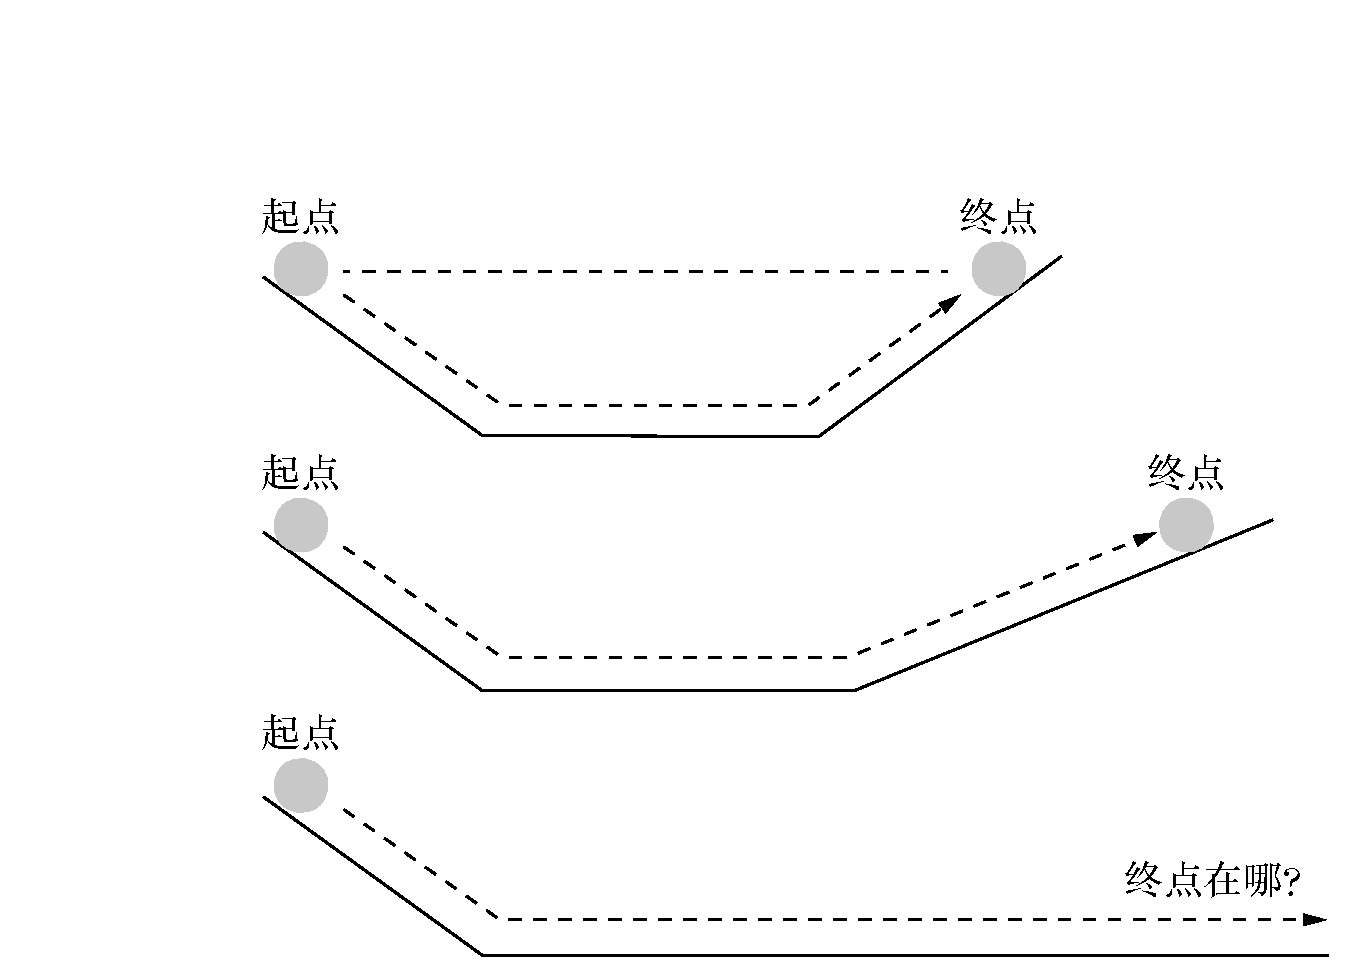
\includegraphics{Galileo}
    \caption{Galileo斜面实验}
    \labfig{Galileo_slope_experiment}
\end{marginfigure}

这个误差就是上面提到的单元内误差.这种误差在是心理学中的一种非常特殊的误差,在物理实验中就不存在这样误差,比如在Galileo的斜面实验(slope experiment),可以看到\reffig{Galileo_slope_experiment}中每个圆球都会上升到同一个高度,不同的球在各种属性上都是完全相同的,所以重复实验对物理属性匹配了的圆球就会有相同效果.但是对于人而言,每个人都不一样,都带着性别、性格、年龄、教育程度等进入实验室,而这些因素会影响行为,我们无法做到匹配完全相同的两个人.
这个变异在完全随机设计中给我们提供了一个随机误差的估计,所有的处理效应都是和它相比,尽管这部分变异不完全是随机的,不过对于完全随机设计而言已经没有更好的办法了.

从这个角度上来说,任何实验中每一组内都不可能只用一个被试,如果只有一个被试就没有变异了,起码两个人才有变异.

\subsection{评价}

完全随机实验设计的\textbf{优点}是,实验设计和实施简单,接受每个处理水平的被试数量可以不相等,不需要匹配被试,每个被试公接受一个处理水平.完全随机实验的统计分析和对结果的解释简单,并且与它的误差平方和相对应的自由度最大。因此,如果在不同的实验设计中得到的误差平方和相等,那么完全随机实验设计比其他实验设计更敏感.

完全随机实验设计的\textbf{缺点}是,它的组内变异并非全部由随机误差组成,其中还包括了被试的个体差异.虽然完全随机设计假设随机分配的各组被试在统计上是无差异的,但实际上被试的个体差异带来的无关变异是存在的,并且混杂在组内变异中,导致$F$比率的分母项加大, 从而使实验较为不敏感.另外,当实验中含多个处理水平时,需要的被试量也会较大.



\section{单因素随机区组实验设计}

\subsection{基本特点}
行为科学研究中,被试的个体差异是误差变异的重要来源.它常常会混淆实验处理效应,因此是无关变异.

方差分析用随机误差代表一些随机发生的因素带来的影响,如果某个效应带来的变异显著大于随因素带来的变异,我们认为这个效应不同于随机因素,是个在统计上有显著意义的效应.然而,在完全随机实验设计中,这个误差的衡量方式是所有被试间的个体差异,但是被试间的个体误差不能完全代表随机误差,因变量对其中某些因素是敏感的.在这些个体差异带来的无关变异中,随机区组设计找出影响因变量最大的,分离这个无关变量带来的变异,使误差效应变小,使这部分无关变异既不出现在处理效应中混淆处理作用的大小,也不出现在误差中降低检验力.这样在$F$检验中:
\[F=\frac{MSA}{MS_{\text{组内}}}\]

将$MSE$中由无关变量$B$带来的无关变异减去,得到
\[MSE=MS_{组内}-MSB\]

使误差效应更小,$F$更容易显著.

单因素随机区组设计适用于这样的情境:研究中有一个自变量,自变量有两个或多个水平$\left( P \geq 2 \right)$,研究中还有一个无关变量,也有两个或多个水平$\left( n \geq 2 \right)$,并且自变量的水平与无关变量的水平之间没有交互作用.

当无关变量是\textbf{被试变量}时, 一般首先将被试在这个无关变量上进行匹配,然后将他们随机分配给不同的实验处理.这样,区组内的被试在此无关变量上更加同质,他们接爱不同的处理水平时,可看作不受无关变量的影响,主要受处理的影响而区组之间的变异反映了无关变量的影响,我们可以利用方差分析技术区分出这一部分变异,经减少误差变异,获得对应效应的更精确估价.

另外环境因素也是潜在可考虑的区组变量,例职,每天的时间、每年的季节、地点、仪器等方面的因素也可以进行区组,经减少误差变异,\textbf{时间}是一个特别有效的区组变量,因为它常常还会带来一些附加自变量,如身体的生理周期、疲劳等.



\begin{margintable}
	\centering
	\caption{单因素随机区组实验设计中被试的分配}
	\labtab{one_way_ANOVA_block_subject}
	{
			\begin{tabular}{ccccc}
			\toprule
			 & $a_1$ & $a_2$ & $a_3$ & $a_4$ \\
			\midrule
			区组1 & $S_1$ & $S_2$ & $S_3$ & $S_4$ \\
			区组2 & $S_5$ & $S_6$ & $S_7$ & $S_8$ \\
			区组3 & $S_9$ & $S_{10}$ & $S_{11}$ & $S_{12}$ \\
			区组4 & $S_{13}$ & $S_{14}$ & $S_{15}$ & $S_{16}$ \\
			\bottomrule
		\end{tabular}	
	}
\end{margintable}

单因素随机区组实验设计中被试与处理的分配如\vreftab{one_way_ANOVA_block_subject},图中可以看出实验中有一个自变量,该自变量有4个水平.实验中还有一个无关变量,将16个被试在无关变量上进行匹配,分为4个区组,每个区组内4个同质被试,随机分配每个被试接受一个处理水平.

单因素随机区组的下标字母与单因素完全随机差不多,不同的是,完全随机设计中,每个处理内被试有多个,故$i$表示的是处理内第$i$个被试,每个处理都有$n$个被试;而在随机区组设计中,不存在这种处理内的被试,我们看到\vreftab{one_way_ANOVA_block_subject}中$a_1$下的4个被试又属于不同的区组.因此,现在的处理内的被试换成了区组,故一共有$n$个区组,$i$表示第$i$个区组.

\subsubsection{单因素随机区组实验设计模型}

\begin{definition}[单因素随机区组设计模型]
\labdef{one_way_ANOVA_block_model}
\begin{align*}
    Y_{ij} = \mu + \alpha _j +  & \pi _i + \varepsilon _{i\left(j\right)}\\
                                & \left( j=1,2,\cdots , p;i = 1,2,\cdots,n \right)
\end{align*}
其中

\begin{tabular}{lcl}
    $Y_{ij}$ & - & 被试在区组$i$和处理水平$j$上的分数 \\
    $\mu$ & - & 总体平均数 \\
    $\alpha _j$ & - & 水平$j$的处理效应 \\
    $\pi _i ^2$ & - & 区组效应,且$\pi _i ^2\sim N\left(0,\sigma _\pi ^2\right)$\\
    $\varepsilon_{i \left( j \right)}$ & - & 误差效应 \\
\end{tabular}
\end{definition}


%
%
%
%
\subsubsection{单因素随机区组实验设计检验的假说}



1.处理水平的总体平均数相等
\[ \mu _{.1} = \mu _{.2} = \cdots = \mu _{.p} \]

或处理效应等于0,即
\[ \alpha _j = 0 \]

2.区组的总体平均数相等
\[ \mu _{1.} = \mu _{2.} = \cdots = \mu _{n.} \]

或区组效应等于0,即
\[ H_0 : \pi _i ^2 = 0\]

因随机区组设计中假设区组变量和自变量间没有交互作用,所以在假设中就没有关于交互作用假设.

\subsection{实验设计和计算举例}
\subsubsection{研究问题}
我们仍利用第一节中文章的生字密度对阅读理解影响的研究做例子,由于考虑到学生的智力可能对阅读理解测验分数产生影响,但它又不是该实验中感兴趣的因素,我决定把学生的智力作为一个无关变量,通过实验设计将它的效应分离出去,以更好地探讨生字密度对阅读理解的影响.我选用了单因素随机区组实验设计.这时,我的研究假说、实验的自变量、因变量都是不变的,只是增加了一个无关变量.在实验实施前,我首选要给32个学生做智力测验,并按智力将学生分为8个区组,然后随机分配每个区组内的4个同质被试分别阅读一种生字密度的文章.

\subsubsection{数据计算}

\textbf{1.计算表}
%----------------------------单因素随机区组设计计算表
\begin{margintable}
	\centering
	\caption{单因素随机区组实验的$AS$表}
	\labtab{one_way_ANOVA_AS_TAB}
	{
		\begin{tabular}{ccccc|c}
			\toprule
    			 & $a_1$ &  $a_2$ &  $a_3$ &  $a_4$ & $\sum$ \\
    			     \midrule
                        区组1 & \cellcolor[rgb]{ .949,  .949,  .949}3 & \cellcolor[rgb]{ .949,  .949,  .949}4 & \cellcolor[rgb]{ .949,  .949,  .949}8 & \cellcolor[rgb]{ .949,  .949,  .949}9 & \cellcolor[rgb]{ .988,  .894,  .839}24 \\
                        区组2 & \cellcolor[rgb]{ .949,  .949,  .949}6 & \cellcolor[rgb]{ .949,  .949,  .949}6 & \cellcolor[rgb]{ .949,  .949,  .949}9 & \cellcolor[rgb]{ .949,  .949,  .949}8 & \cellcolor[rgb]{ .988,  .894,  .839}29 \\
                        区组3 & \cellcolor[rgb]{ .949,  .949,  .949}4 & \cellcolor[rgb]{ .949,  .949,  .949}4 & \cellcolor[rgb]{ .949,  .949,  .949}8 & \cellcolor[rgb]{ .949,  .949,  .949}8 & \cellcolor[rgb]{ .988,  .894,  .839}24 \\
                        区组4 & \cellcolor[rgb]{ .949,  .949,  .949}3 & \cellcolor[rgb]{ .949,  .949,  .949}2 & \cellcolor[rgb]{ .949,  .949,  .949}7 & \cellcolor[rgb]{ .949,  .949,  .949}7 & \cellcolor[rgb]{ .988,  .894,  .839}19 \\
                        区组5 & \cellcolor[rgb]{ .949,  .949,  .949}5 & \cellcolor[rgb]{ .949,  .949,  .949}4 & \cellcolor[rgb]{ .949,  .949,  .949}5 & \cellcolor[rgb]{ .949,  .949,  .949}12 & \cellcolor[rgb]{ .988,  .894,  .839}26 \\
                        区组6 & \cellcolor[rgb]{ .949,  .949,  .949}7 & \cellcolor[rgb]{ .949,  .949,  .949}5 & \cellcolor[rgb]{ .949,  .949,  .949}6 & \cellcolor[rgb]{ .949,  .949,  .949}13 & \cellcolor[rgb]{ .988,  .894,  .839}31 \\
                        区组7 & \cellcolor[rgb]{ .949,  .949,  .949}5 & \cellcolor[rgb]{ .949,  .949,  .949}3 & \cellcolor[rgb]{ .949,  .949,  .949}7 & \cellcolor[rgb]{ .949,  .949,  .949}12 & \cellcolor[rgb]{ .988,  .894,  .839}27 \\
                        区组8 & \cellcolor[rgb]{ .949,  .949,  .949}2 & \cellcolor[rgb]{ .949,  .949,  .949}3 & \cellcolor[rgb]{ .949,  .949,  .949}6 & \cellcolor[rgb]{ .949,  .949,  .949}11 & \cellcolor[rgb]{ .988,  .894,  .839}22 \\
                        \midrule
                              $\sum$ & \cellcolor[rgb]{ .886,  .937,  .855}35 & \cellcolor[rgb]{ .886,  .937,  .855}31 & \cellcolor[rgb]{ .886,  .937,  .855}56 & \cellcolor[rgb]{ .886,  .937,  .855}80 & \cellcolor[rgb]{ .867,  .922,  .969}202 \\

			\bottomrule
		\end{tabular}
	}
\end{margintable}
%----------------------------------------------------------------------------
\textbf{2.各种基本量的计算}
    \begin{align*}
        %----------------------------------------------------------
        %[Y]
            \frac{
                \left(
        	\sum\limits_{i=1}^{n} \sum\limits_{j=1}^{p}Y_{ij}
                \right)^2}
            {np}=& \colorbox[rgb]{ .867,  .922,  .969}{$[Y]$} = 
            \frac{
                \left(
        	    202
                \right)^2}
                {
                    \left(
        	           8
                    \right)^2
                    \left(
                        4
                    \right)^2
                }&=1275.125\\
        %----------------------------------------------------------
        %[AS]
            \sum\limits_{i=1}^{n} \sum\limits_{j=1}^{p}Y_{ij}^2=
            & \colorbox[rgb]{ .949,  .949,  .949}{$[AS]$} = 
            \left(
            	3
            \right)^2 +
            \left(
            	6
            \right)^2    +\cdots &=1544.000\\
        %----------------------------------------------------------
        %[A]    
            \sum\limits_{i=1}^{n}
            \frac
                {\left(
	            \sum\limits_{j=1}^{p}Y_{ij}
                \right)^2}
                {n}=
            &\colorbox[rgb]{ .886,  .937,  .855}{$[A]$}=
            \frac{\left(35\right)^2}{8}+\frac{\left(31\right)^2}{8}+\cdots&=1465.250\\
        %---------------------------------------------------------
        %[S]
            \sum\limits_{i=1}^{n}
            \frac
            {
                \sum\limits_{j=1}^{p}\left(Y_{ij} \right)^2
            }
            {
                p            
            }            
            =&\colorbox[rgb]{ .988,  .894,  .839}{$[S]$}
            =\frac{\left( 24 \right)^2}{4} + \frac{\left( 29 \right)^2}{4} + \cdots &= 1301.000
    \end{align*}
%---------------------------------------------
\textbf{3.平方和的分解}

\begin{definition}[单因素随机区组设计平方和的分解]
\labdef{one_way_ANOVA_block_variance_breakthrough}
\begin{alignat*}{2}
   & SS_{\text{总变异}} &&= SS_{\text{处理间}} + SS_{\text{处理内}}\\
   &                    &&= SSA + (SS_{\text{区组}} + SS_{\text{残差}})
\end{alignat*}
\end{definition}
\begin{alignat*}{3}
    &    SS_{\text{总变异}} &&     =[AS]-[Y]                                 && =268.875\\
    &    SSA                &&    =[A]-[Y]                                  && =190.125\\
    &    SS_{\text{区组}}   &&    =[S]-[Y]                                   && =25.750\\
    &    SS_{\text{残差}}   &&    =SS_{\text{总变异}}-SSA-SS_{\text{区组}}    &&=52.875
\end{alignat*}
%----------------------
\textbf{4.方差分析表及结果解释}
\begin{table}[h]
	\centering
	\caption{单因素随机区组实验的方差分析表}
	\labtab{one_way_block_ANOVA_Tab}
	{
		\begin{tabular}{lrrcrrr}
			\toprule
			\multicolumn{1}{c}{变异源} & \multicolumn{1}{c}{$SS$} & \multicolumn{1}{c}{$df$} & \multicolumn{1}{c}{$MS$} & \multicolumn{1}{c}{$F$} & \multicolumn{1}{c}{$p$} \\
			\midrule
			$A$(生字密度) & 190.125 & $p-1=3$ & 63.375 & 25.170 & $<$ .001  \\
			区组(智力) & 25.850 & $n-1=7$ & 3.696 & 1.47 & 0.23   \\
			残差 & 52.875 & $(n-1)(p-1)=21$ & 2.518\\
			\midrule
			总计 & 268.875 & $np-1=31$ & & &\\
			\bottomrule
			% \addlinespace[1ex]
			% \multicolumn{6}{p{0.5\linewidth}}{\textit{Note.} Type III Sum of Squares} \\
		\end{tabular}
	}
\end{table}

方差分析可以看出,实验中的自变量——生字密度的效应是统计显著的$\left( F(3,21)=25.170, p < .001 \right)$,说明学生对生字密度不同的文章的阅读理解有显著差别.实验中无关变量——智力的效应是统计上不显著的$\left( F \left( 7,21 \right) = 1.47, p > .05 \right)$,表明本实验中智力不同的学生的阅读理解 没有明显差异.方差分析表中还可以看出,生字密度和智力的$F$检验都使用了同一个误差项$MSE=2.518$.

\textbf{5.平方和与自由度分解图}


\subsection{一些解释}
\textbf{1.各种平方和的意义}

\begin{description}
\item[$SS_{\text{总变异}}$]——在随机区组实验中,总平方和应首先分解为处理间平方和处理内平方和应首先分解 为处理间平方和处理内平方和.
\item[$SS_{\text{处理间}}$]——处理间平方和指所有由实验处理引起的变异,在单因素设计中指$A$因素的处理效应$SSA$
\item[$SS_{\text{处理内}}$]——在随机区组实验中,处理内平方和可进一步分解为两部分:区组平方和和误差平方和.
\item[$SS_{\text{区组}}$]——区组效应,在该实验中指总变异中由被试的智力引起的变异.
\item[$SS_{\text{残差}}$]——残差指总变异中不能被实验处理和区组效应解释的变异.在随机区组实验设计中,接受同实验条件的同质被试只有一个,因此,不能计算单元内误差,而残差作为误差变异的估计.残差的计算是从总变异中减去处理效应和区组变异.
\end{description}

\textbf{2.做区组的方法}

除了感兴趣的自变量外,还有很多无关就量都影响因变量.如果发现一个变量特别影响因变量,但对其效应不感兴趣,可以考虑将其作一个区组.本例中区组变量是智力,我们知道一个孩子的智力情况会影响他的阅读理解,如果一个组里都是智力低的孩子,一个组里都是智力高的孩子.若智力高的组分配的是低生字密度,生字密度和智力都会促进阅读理解,处理效应被加大,当本身处理效应不显著时,会面临错误判定处理效应显著的失误;若智力高的组分配的是高生字密度,自变量效应方向和无关变量方向相反,它们抵消后会使处理效应被掩盖,造成处理效应不显著.

\textbf{3.随机区组提高实验敏感性的体现}

前面我提到从$F$值的大小思考实验的敏感性,单因素完全随机的$F$值:
\[ F=\frac{MSA}{MS_{\text{组内}}} \]

单因素随机区组设计将$SS_{组内}$进一步分解为$SS_{\text{区组}}$和$SS_{\text{残差}}$,既然区组变量带来的变异不是随机误差,因此将其从组内误差中分离出来,这样误差项就减小了,从而单因素随机区组的$F$值就是:
\[ F = \frac{MSA}{MS_{\text{残差}}} \]

而$MS_{\text{残差}} < MS_{\text{组内}}$,因而提升了实验的敏感性.从数据上,我们可以看到,在\vreftab{one_way_ANOVA_Tab}中,组内误差是78.750,在同样的数据用了随机区组的算法后,\vreftab{one_way_block_ANOVA_Tab}中可以看出,将组内误差分解成了区组带来的无关变异25.850,和剩余的残差52.875.完全随机的$F$是22.533,在随机区组中$F$是25.170,这看上去没有提升多少,原因是这组数据中区组变量的效应是不显著的,可以看到残差项还是很大,说明这个随机区组变量并不是特别有效.

那么什么是有效的随机区组设计呢?
在\vreftab{one_way_ANOVA_AS_TAB}中右边红色的数据是对把自变量处理水平$a_1,a_2,a_3,a_4$合并起来的数据,这样这个数据只和集中趋势和区组无关变量带来的变异相关,我们把它按小到大排个序:
\[ 19,22,24,24,26,27,29,21 \]

这和绿色的数据:
\[ 31,35,56,80 \]

相比,变异就小了很多.一个好的区组设计应该让红色的那部分数据呈现一个明显的梯度,让它们之间相差得大一点,这样就可以带走更多变异.这点不是实验操作上可以保证的,主要是要看这个区组变量是不是一个有效的区组变量,是否对因变量有较大影响.

\textbf{4.残差的实质}

从方差分析中的自由度(见\vreftab{one_way_block_ANOVA_Tab})知,残差的自由度是$(p-1)(n-1)$,这个形式表明这个残差本质是个交互作用.现在还不是时候从根本上揭示残差的实质.

随机区组中,用残差来估价随机误差,今后我们将看到,所有的误差项只有两种形式,一种是单元内误差(当有同质被试接受相同的处理时产生),一种是残差(实验是交互作用).在随机区组设计中,由于没有接受相同处理的同质被试,故不存在单元内误差.

\subsection{评价}
随机区组的\textbf{优点}是,在许多研究情境中,它比完全随机实验设计更加有效.这是由于它使研究者从总变异中分离出了一个无关变量的效应,从而减小了实验误差,可获得对处理效应的更加精确的估价.随机区组实验设计可使用于含任何处理水平数的实验中,并且区组的数量也不受限制,因而有较好的灵活性.

随机区组实验设计的\textbf{缺点}是,如实验中含有多处理水平,可能给形成同质区组、寻找同质被试带来困难.另外,使用随机区组设计比使用完全随机设计有更多的限定,例如使用随机区组实验设计的前提假设是,实验中的自变量与无关变量之间没有交互作用.如果交互作用是存在的,使用随机区组实验设计是不合适的.这在一定程度上限制了随机区组实验设计的应用.但由于无法对该残差的显著性进行检验,故对于这个误差的估计是否合理就没有检验的方法.

\subsection{经典随机区组设计的改进}
\subsubsection{基本思想}
经典随机区组设计中,误差用残差衡量,它的实质是区组变量与自变量间的交互作用,问题是我们无法保证它们间一定不存在交互作用,我们甚至没有检验这个交互作用显著性的手段.

单元内误差是一定是一个可靠的误差估计,不过在经典随机区组设计中没有接受相同处理的同质被试,那对其进行改进即可,让区组内人数扩大,使接受同一个处理和在同一个区组内的被试有多个,这样可以算出单元内误差,检验残差是否显著.

\subsubsection{评价}
我们力求区组内被试同质,但是实际上很难做到.本例来说,区组变量是智力,这是一个连续变量.增加区组内被试时,有很大可有使区组内的变异变大,很有可能让区组间的变小.

所以随机区组设计不会用这种方式.

\section{单因素拉丁方实验设计}

拉丁方设计最大特色是同时计算了残差和单元内误差,扩展了区组实验设计.对于完全随机方差分析中的$F$检验而言:
\[ F=\frac{MSA}{MS_{\text{组内}}} \qquad MS_{\text{组内}}=\text{无关变异}+\text{随机误差} \]

由于完全随机设计中误差项$MSE$中混入了个体差异和一些其它的无关变异,所以随机区组设计找到一个影响较大的无关变异,计算其大小并从$MSE$中分离,这样新的$MSE$就等于$MSE_{\text{组内}}-MS_{\text{区组}}$,误差项减小,可以提高实验的精度.
不过这样还不够,首先,对于影响因变量的无关变量不止有一个,也许除了生字密度学、生的智力外,还有别的无关变量对阅读理解有较大影响.故我们希望可以再分离出一个无关变量的效应;
其次,随机区组的误差是否是一个合理的误差也不清楚
所以我还希望在每一个区组内加入多个被试,以检验残差的是否显著.

总的来说,拉丁方实验设计同时分离两个无关变量的效应,同时通过分配多个被试给同一自变量水平和无关变量水平的结合,使得可以计算出单元内误差来检验残差是否显著.不过该设计对两个无关变量有较大要求.拉丁方实验设计适合下列条件:

\begin{description}
\item[1.自变量和无关变量的水平限制] 自变量的水平和两个无关变量的水平相等,即自变量水平是$p$ $(p\geq 2)$,两个无关变量水平都是$p$ $(p\geq 2)$;
\item[2.自变量与无关变量无交互作用] 如果这个假设不能满足峄实验中的一个或多个效应的检验可能有偏差
\item[3.拉丁方限制]随机分配处理立平给$p^2$个方格单元,每个处理水平仅在每行、每列中出现一次
\end{description}

%-----------begin连续的拉丁方快
\begin{margintable}
  \caption{$2\times 2$拉丁方快}
  \labtab{lantin_square_2_2}
    \begin{tabular}{cc}
    A     & B \\
    B     & A \\
    \end{tabular}
\end{margintable}

\begin{margintable}
  \caption{$3\times 3$拉丁方快}
  \labtab{lantin_square_3_3}
    \begin{tabular}{ccc}
    A  &  B  &  C\\
    B  &  C  &  A\\
    C  &  A  &  B\\
    \end{tabular}
\end{margintable}

\begin{margintable}
  \caption{$4\times 4$拉丁方快}
  \labtab{lantin_square_4_4}
    \begin{tabular}{cccc}
    A     & B     & C     & D \\
    B     & C     & D     & A \\
    C     & D     & A     & B \\
    D     & A     & B     & C \\
    \end{tabular}
\end{margintable}

\begin{margintable}
  \caption{$5\times 5$拉丁方快}
  \labtab{lantin_square_5_5}
    \begin{tabular}{ccccc}
    A     & B     & C     & D     & E \\
    B     & C     & D     & E     & A \\
    C     & D     & E     & A     & B \\
    D     & E     & A     & B     & C \\
    E     & A     & B     & C     & D \\
    \end{tabular}
\end{margintable}
%---------------------end连续的拉丁方快

我列出了五个拉丁方格:\vreftab{lantin_square_2_2},\vreftab{lantin_square_3_3},\vreftab{lantin_square_4_4},\vreftab{lantin_square_5_5},从列子中可以看到拉丁方格每一行每一列每一个字母只出现一次,下面以$4\times 4$拉丁方表格介绍一下拉丁方格随机化的方法:

\begin{table}[h]
  \caption{拉丁方格标准化方块的随机化}
  \labtab{lantin_square_norm}
    \begin{tabular}{ccccccccccc}
          & \multicolumn{4}{c}{标准块}       &       &       & \multicolumn{4}{c}{随机化行} \\
          & 1     & 2     & 3     & 4     &       &       & 1     & 2     & 3     & 4 \\
    1     & \cellcolor[rgb]{ .851,  .882,  .949}A & \cellcolor[rgb]{ .851,  .882,  .949}B & \cellcolor[rgb]{ .851,  .882,  .949}C & \cellcolor[rgb]{ .851,  .882,  .949}D &       & 3     & \cellcolor[rgb]{ .886,  .937,  .855}C & \cellcolor[rgb]{ .886,  .937,  .855}D & \cellcolor[rgb]{ .886,  .937,  .855}A & \cellcolor[rgb]{ .886,  .937,  .855}B \\
    2     & \cellcolor[rgb]{ 1,  .949,  .8}B & \cellcolor[rgb]{ 1,  .949,  .8}C & \cellcolor[rgb]{ 1,  .949,  .8}D & \cellcolor[rgb]{ 1,  .949,  .8}A &       & 1     & \cellcolor[rgb]{ .851,  .882,  .949}A & \cellcolor[rgb]{ .851,  .882,  .949}B & \cellcolor[rgb]{ .851,  .882,  .949}C & \cellcolor[rgb]{ .851,  .882,  .949}D \\
    3     & \cellcolor[rgb]{ .886,  .937,  .855}C & \cellcolor[rgb]{ .886,  .937,  .855}D & \cellcolor[rgb]{ .886,  .937,  .855}A & \cellcolor[rgb]{ .886,  .937,  .855}B &       & 2     & \cellcolor[rgb]{ 1,  .949,  .8}B & \cellcolor[rgb]{ 1,  .949,  .8}C & \cellcolor[rgb]{ 1,  .949,  .8}D & \cellcolor[rgb]{ 1,  .949,  .8}A \\
    4     & \cellcolor[rgb]{ .929,  .929,  .929}D & \cellcolor[rgb]{ .929,  .929,  .929}A & \cellcolor[rgb]{ .929,  .929,  .929}B & \cellcolor[rgb]{ .929,  .929,  .929}C &       & 4     & \cellcolor[rgb]{ .929,  .929,  .929}D & \cellcolor[rgb]{ .929,  .929,  .929}A & \cellcolor[rgb]{ .929,  .929,  .929}B & \cellcolor[rgb]{ .929,  .929,  .929}C \\
          &       &       &       &       &       &       &       &       &       &  \\
          & \multicolumn{4}{c}{随机化行}      &       &       & \multicolumn{4}{c}{随机化列} \\
          & 1     & 2     & 3     & 4     &       &       & 4     & 3     & 1     & 2 \\
    3     & \cellcolor[rgb]{ .851,  .882,  .949}C & \cellcolor[rgb]{ .988,  .894,  .839}D & \cellcolor[rgb]{ .929,  .929,  .929}A & \cellcolor[rgb]{ .886,  .937,  .855}B &       & 3     & \cellcolor[rgb]{ .886,  .937,  .855}B & \cellcolor[rgb]{ .929,  .929,  .929}A & \cellcolor[rgb]{ .851,  .882,  .949}C & \cellcolor[rgb]{ .988,  .894,  .839}D \\
    1     & \cellcolor[rgb]{ .851,  .882,  .949}A & \cellcolor[rgb]{ .988,  .894,  .839}B & \cellcolor[rgb]{ .929,  .929,  .929}C & \cellcolor[rgb]{ .886,  .937,  .855}D &       & 1     & \cellcolor[rgb]{ .886,  .937,  .855}D & \cellcolor[rgb]{ .929,  .929,  .929}C & \cellcolor[rgb]{ .851,  .882,  .949}A & \cellcolor[rgb]{ .988,  .894,  .839}B \\
    2     & \cellcolor[rgb]{ .851,  .882,  .949}B & \cellcolor[rgb]{ .988,  .894,  .839}C & \cellcolor[rgb]{ .929,  .929,  .929}D & \cellcolor[rgb]{ .886,  .937,  .855}A &       & 2     & \cellcolor[rgb]{ .886,  .937,  .855}A & \cellcolor[rgb]{ .929,  .929,  .929}D & \cellcolor[rgb]{ .851,  .882,  .949}B & \cellcolor[rgb]{ .988,  .894,  .839}C \\
    4     & \cellcolor[rgb]{ .851,  .882,  .949}D & \cellcolor[rgb]{ .988,  .894,  .839}A & \cellcolor[rgb]{ .929,  .929,  .929}B & \cellcolor[rgb]{ .886,  .937,  .855}C &       & 4     & \cellcolor[rgb]{ .886,  .937,  .855}C & \cellcolor[rgb]{ .929,  .929,  .929}B & \cellcolor[rgb]{ .851,  .882,  .949}D & \cellcolor[rgb]{ .988,  .894,  .839}A \\
    \end{tabular}%
\end{table}

单因素拉丁方实验设计被试分配到处理上的例子如\vreftab{latin_subject_treatment}.从表中可以看出,实验中的自变量$A$有4个水平,无关变量$B$和无关变量$C$也各有4个水平,形成$4\times 4$的拉丁方格,32个被试参加了实验,每个方格内有2个被试,每个被试只接受一种独特的实验条件处理.

\begin{margintable}
  \centering
  \caption{单因素拉丁方实验设计中被试的分配}
    \begin{tabular}{ccccc}
          & $c_1$ & $c_2$ & $c_3$ & $c_4$ \\
    \multirow{3}[0]{*}{$b_1$} & \cellcolor[rgb]{ .851,  .882,  .949}$a_1$ & \cellcolor[rgb]{ .851,  .882,  .949}$a_2$ & \cellcolor[rgb]{ .851,  .882,  .949}$a_3$ & \cellcolor[rgb]{ .851,  .882,  .949}$a_4$ \\
          & \cellcolor[rgb]{ .886,  .937,  .855}$S_1$ & \cellcolor[rgb]{ .886,  .937,  .855}$S_9$ & \cellcolor[rgb]{ .886,  .937,  .855}$S_{17}$ & \cellcolor[rgb]{ .886,  .937,  .855}$S_{25}$ \\
          & \cellcolor[rgb]{ .886,  .937,  .855}$S_2$ & \cellcolor[rgb]{ .886,  .937,  .855}$S_{10}$ & \cellcolor[rgb]{ .886,  .937,  .855}$S_{18}$ & \cellcolor[rgb]{ .886,  .937,  .855}$S_{26}$ \\
    \multirow{3}[0]{*}{$b_2$} & \cellcolor[rgb]{ .851,  .882,  .949}$a_2$ & \cellcolor[rgb]{ .851,  .882,  .949}$a_3$ & \cellcolor[rgb]{ .851,  .882,  .949}$a_4$ & \cellcolor[rgb]{ .851,  .882,  .949}$a_1$ \\
          & \cellcolor[rgb]{ .886,  .937,  .855}$S_3$ & \cellcolor[rgb]{ .886,  .937,  .855}$S_{11}$ & \cellcolor[rgb]{ .886,  .937,  .855}$S_{19}$ & \cellcolor[rgb]{ .886,  .937,  .855}$S_{27}$ \\
          & \cellcolor[rgb]{ .886,  .937,  .855}$S_4$ & \cellcolor[rgb]{ .886,  .937,  .855}$S_{12}$ & \cellcolor[rgb]{ .886,  .937,  .855}$S_{20}$ & \cellcolor[rgb]{ .886,  .937,  .855}$S_{28}$ \\
    \multirow{3}[0]{*}{$b_3$} & \cellcolor[rgb]{ .851,  .882,  .949}$a_3$ & \cellcolor[rgb]{ .851,  .882,  .949}$a_4$ & \cellcolor[rgb]{ .851,  .882,  .949}$a_1$ & \cellcolor[rgb]{ .851,  .882,  .949}$a_2$ \\
          & \cellcolor[rgb]{ .886,  .937,  .855}$S_5$ & \cellcolor[rgb]{ .886,  .937,  .855}$S_{13}$ & \cellcolor[rgb]{ .886,  .937,  .855}$S_{21}$ & \cellcolor[rgb]{ .886,  .937,  .855}$S_{29}$ \\
          & \cellcolor[rgb]{ .886,  .937,  .855}$S_6$ & \cellcolor[rgb]{ .886,  .937,  .855}$S_{14}$ & \cellcolor[rgb]{ .886,  .937,  .855}$S_{22}$ & \cellcolor[rgb]{ .886,  .937,  .855}$S_{30}$ \\
    \multirow{3}[0]{*}{$b_4$} & \cellcolor[rgb]{ .851,  .882,  .949}$a_4$ & \cellcolor[rgb]{ .851,  .882,  .949}$a_1$ & \cellcolor[rgb]{ .851,  .882,  .949}$a_2$ & \cellcolor[rgb]{ .851,  .882,  .949}$a_3$ \\
          & \cellcolor[rgb]{ .886,  .937,  .855}$S_7$ & \cellcolor[rgb]{ .886,  .937,  .855}$S_{15}$ & \cellcolor[rgb]{ .886,  .937,  .855}$S_{23}$ & \cellcolor[rgb]{ .886,  .937,  .855}$S_{31}$ \\
          & \cellcolor[rgb]{ .886,  .937,  .855}$S_8$ & \cellcolor[rgb]{ .886,  .937,  .855}$S_{16}$ & \cellcolor[rgb]{ .886,  .937,  .855}$S_{24}$ & \cellcolor[rgb]{ .886,  .937,  .855}$S_{32}$ \\
    \end{tabular}%
  \labtab{latin_subject_treatment}
\end{margintable}

\begin{definition}[单因素拉丁方设计模型]
\labdef{one_way_latin_model}
\begin{align*}
    Y_{ijkl} = \mu + \alpha _j + \beta _k & + \gamma _l + \varepsilon _{pooled}\\
                                          &(j=1,2,\cdots,p;i=1,2,\cdots,n)\\
                                          &(k=1,2,\cdots,p;l=1,2,\cdots,p)
\end{align*}

其中

\begin{tabular}{ccl}
    $Y_{ijkl}$     & - &    两无关变量在第$j,k$个水平上,被试$i$的分数\\ 
    $\mu$          & - &    总体平均值或真值\\
    $\alpha _j$    & - &    自变量水平$j$的处理效应\\
    $\beta _k$     & - &    无关变量$B$水平$k$的变异\\
    $\gamma _l$    & - &    无关变量$C$水平$l$的变异\\
    $\varepsilon _{pooled}$ &-& 合并误差
\end{tabular}

\end{definition}

模型中的$\varepsilon _{pooled}$,pooled指的是“集合的,集中的”,这是两项误差的合并,这点我在后面会介绍.

拉丁方实验设计适合检验的假说是:

(1)处理水平的总体平均数相等,即:
\[ H_0 : \mu _{1..} = \mu _{2..} = \cdots = \mu _{p..}\]

或因素$A$效应等于0,即:
\[ H_0 : \alpha _j = 0 \]

(2)无关变量(横行)的总体平均数相等,即
\[ H_0 : \mu _{.1.} = \mu _{.2.} = \cdots = \mu _{.p.} \]

或无关变量$B$的效应等于0,即
\[ \beta _k = 0 \]

(3)无关变量(纵行)的总体平均数相等,即
\[ H_0 : \mu _{..1} = \mu _{..2} = \cdots = \mu _{..p} \]

或无关变量$C$的效应等于0,即
\[ \gamma _l = 0 \]




 \subsection{实验设计与计算举例}
 
 \subsubsection{研究的问题与实验设计}
 
 \subsubsection{实验数据及其计算}

\textbf{计算表}

%---ABCS表--------------------------------------------------------------
\begin{margintable}
  \centering
  \caption{拉丁方设计$ABCS$表}
    \begin{tabular}{ccccc}
    \toprule
          & $c_1$ & $c_2$ & $c_3$ & $c_4$ \\
    \midrule
          & $a_1$ & $a_2$ & $a_3$ & $a_4$ \\
    \multirow{2}[0]{*}{$b_1$} & \cellcolor[rgb]{ .949,  .949,  .949}3 & \cellcolor[rgb]{ .949,  .949,  .949}2 & \cellcolor[rgb]{ .949,  .949,  .949}6 & \cellcolor[rgb]{ .949,  .949,  .949}9 \\
          & \cellcolor[rgb]{ .949,  .949,  .949}4 & \cellcolor[rgb]{ .949,  .949,  .949}3 & \cellcolor[rgb]{ .949,  .949,  .949}5 & \cellcolor[rgb]{ .949,  .949,  .949}8 \\
          & $a_2$ & $a_3$ & $a_4$ & $a_1$ \\
    \multirow{2}[0]{*}{$b_2$} & \cellcolor[rgb]{ .949,  .949,  .949}8 & \cellcolor[rgb]{ .949,  .949,  .949}3 & \cellcolor[rgb]{ .949,  .949,  .949}4 & \cellcolor[rgb]{ .949,  .949,  .949}7 \\
          & \cellcolor[rgb]{ .949,  .949,  .949}7 & \cellcolor[rgb]{ .949,  .949,  .949}2 & \cellcolor[rgb]{ .949,  .949,  .949}3 & \cellcolor[rgb]{ .949,  .949,  .949}6 \\
          & $a_3$ & $a_4$ & $a_1$ & $a_2$ \\
    \multirow{2}[0]{*}{$b_3$} & \cellcolor[rgb]{ .949,  .949,  .949}8 & \cellcolor[rgb]{ .949,  .949,  .949}12 & \cellcolor[rgb]{ .949,  .949,  .949}5 & \cellcolor[rgb]{ .949,  .949,  .949}6 \\
          & \cellcolor[rgb]{ .949,  .949,  .949}9 & \cellcolor[rgb]{ .949,  .949,  .949}13 & \cellcolor[rgb]{ .949,  .949,  .949}6 & \cellcolor[rgb]{ .949,  .949,  .949}4 \\
          & $a_4$ & $a_1$ & $a_2$ & $a_3$ \\
    \multirow{2}[0]{*}{$b_4$} & \cellcolor[rgb]{ .949,  .949,  .949}5 & \cellcolor[rgb]{ .949,  .949,  .949}8 & \cellcolor[rgb]{ .949,  .949,  .949}12 & \cellcolor[rgb]{ .949,  .949,  .949}7 \\
          & \cellcolor[rgb]{ .949,  .949,  .949}4 & \cellcolor[rgb]{ .949,  .949,  .949}7 & \cellcolor[rgb]{ .949,  .949,  .949}11 & \cellcolor[rgb]{ .949,  .949,  .949}5 \\
        \bottomrule
    \end{tabular}
  \labtab{latin_square_ABCS_tab}
\end{margintable}

%-----------------------------------------------------------------

%---ABC表
\begin{margintable}
  \centering
  \caption{拉丁方设计$ABC$表}

    \begin{tabular}{ccccc|c}
    \toprule
          & $c_1$ & $c_2$ & $c_3$ & $c_4$ & $\sum$ \\
    \midrule
          & $n=2$ &       &       &       &  \\
          & $a_1$ & $a_2$ & $a_3$ & $a_4$ &  \\
    $b_1$ & \cellcolor[rgb]{ .886,  .937,  .855}7 & \cellcolor[rgb]{ .886,  .937,  .855}5 & \cellcolor[rgb]{ .886,  .937,  .855}11 & \cellcolor[rgb]{ .886,  .937,  .855}17 & \cellcolor[rgb]{ 1,  .949,  .8}40 \\
          & $a_2$ & $a_3$ & $a_4$ & $a_1$ &  \\
    $b_2$ & \cellcolor[rgb]{ .886,  .937,  .855}15 & \cellcolor[rgb]{ .886,  .937,  .855}5 & \cellcolor[rgb]{ .886,  .937,  .855}7 & \cellcolor[rgb]{ .886,  .937,  .855}13 & \cellcolor[rgb]{ 1,  .949,  .8}40 \\
          & $a_3$ & $a_4$ & $a_1$ & $a_2$ &  \\
    $b_3$ & \cellcolor[rgb]{ .886,  .937,  .855}17 & \cellcolor[rgb]{ .886,  .937,  .855}25 & \cellcolor[rgb]{ .886,  .937,  .855}11 & \cellcolor[rgb]{ .886,  .937,  .855}10 & \cellcolor[rgb]{ 1,  .949,  .8}63 \\
          & $a_4$ & $a_1$ & $a_2$ & $a_3$ &  \\
    $b_4$ & \cellcolor[rgb]{ .886,  .937,  .855}9 & \cellcolor[rgb]{ .886,  .937,  .855}15 & \cellcolor[rgb]{ .886,  .937,  .855}23 & \cellcolor[rgb]{ .886,  .937,  .855}12 & \cellcolor[rgb]{ 1,  .949,  .8}59 \\
    $\sum$ & \cellcolor[rgb]{ .839,  .863,  .894}48 & \cellcolor[rgb]{ .839,  .863,  .894}50 & \cellcolor[rgb]{ .839,  .863,  .894}52 & \cellcolor[rgb]{ .839,  .863,  .894}52 & \cellcolor[rgb]{ .867,  .922,  .969}202 \\
    \bottomrule
    \end{tabular}

  \labtab{latin_square_ABC_tab}
\end{margintable}


%---------A表
\begin{margintable}
  \centering
  \caption{拉丁方设计$A$表}
    \begin{tabular}{cccc}
    \toprule
    \multicolumn{1}{c}{$a_1$} & \multicolumn{1}{c}{$a_2$} & \multicolumn{1}{c}{$a_3$} & \multicolumn{1}{c}{$a_4$} \\
    \midrule
    \multicolumn{1}{l}{$np=8$} &       &       &  \\
    \rowcolor[rgb]{ .957,  .69,  .518} 35    & 31    & 56    & 80 \\
    \bottomrule
    \end{tabular}
  \labtab{latin_square_A_tab}
\end{margintable}

\textbf{2.各种基本量的计算}

\begin{align*}
    \sum\limits_{i=1}^{n}\sum\limits_{k=l}^{p}\sum\limits_{l=1}^{p}Y_{ijkl}&=3+4+\cdots=202.000\\
    \frac{\sum\limits_{l=1}^p{\sum\limits_{k=1}^p{\sum\limits_{i=1}^n{Y_{ijkl}}}}}{np^2}=\left[ Y \right] &=\frac{\left( 202 \right) ^2}{\left( 2 \right) \left( 4 \right) ^2}\\
    \sum\limits_{l=1}^p{\sum\limits_{k=1}^p{\sum\limits_{i=1}^n{\left( Y_{ijkl}^{2} \right)}}}&=\left[ ABCS \right] =\left( 3 \right) ^2+\left( 4 \right) ^2+\cdots =1544.000\\
    \sum\limits_{l=1}^p{\sum\limits_{k=1}^p{\frac{\left( \sum\limits_{i=1}^n{Y_{ijkl}} \right) ^2}{n}}}&=\left[ ABC \right] =\frac{\left( 7 \right) ^2}{2}+\frac{\left( 5 \right) ^2}{2}+\cdots =1533.000\\
     &=\left[ A \right] =\frac{\left( 35 \right) ^2}{8}+\frac{\left( 31 \right) ^2}{8}+\cdots =1465.250\\
    \sum\limits_{k=1}^p{\frac{\left( \sum\limits_{l=1}^p{\sum\limits_{i=1}^n{Y_{ijkl}}} \right) ^2}{np}}&=\left[ B \right] =\frac{\left( 40 \right) ^2}{8}+\frac{\left( 40 \right) ^2}{8}+\cdots =1331.250\\
    \sum\limits_{l=1}^p{\frac{\left( \sum\limits_{k=1}^p{\sum\limits_{i=1}^n{Y_{ijkl}}} \right) ^2}{np}}&=\left[ C \right] =\frac{\left( 48 \right) ^2}{8}+\frac{\left( 50 \right) ^2}{8}+\cdots =1276.500\\
\end{align*}


\texfbf{3.平方和分解与计算}
\begin{alignat*}{4}
   & SS_{\text{总变异}} & &= SS_{\text{处理间}} & & +SS_{\text{处理内}}\\
   &                    & &= SSA               & & +\left( SSB + SSC + SS_{\text{单元内}} + SS_{\text{残差}}  \right)
\end{alignat*}


\begin{alignat*}{3}
    & SS_{\text{总变异}} && =[ABCS]-[Y] && =268.875\\
    & SSA               &&  =[A]   - [Y] && =190.125\\
    &SSB               && =[B] -[Y]&&=56.125\\
    & SSC              && =[C]-[Y] &&= 1.375\\
    & SS_{\text{残差}} && = {[ABC]-[Y]}-SSA-SSB-SSC && =10.250\\
    & SS_{\text{单元内}} && = SS_{\text{总变异}}-SSA-SSB-SSC-SS_{\text{残差}} && = 11.000
\end{alignat*}


\textbf{4.方差分析表及对结果的解释}

\begin{table}[h]
	\centering
	\caption{单因素拉丁方实验的方差分析表}
	\labtab{one_way_latin_ANOVA_Tab}
	{
		\begin{tabular}{lrrcrrr}
			\toprule
			\multicolumn{1}{c}{变异源} & \multicolumn{1}{c}{$SS$} & \multicolumn{1}{c}{$df$} & \multicolumn{1}{c}{$MS$} & \multicolumn{1}{c}{$F$} & \multicolumn{1}{c}{$p$} \\
			\midrule
			A(生字密度) & 190.125 & $p-1=3$ & 63.375 & 25.170 & $<$.001  \\
			B(班级) & 56.125 & $p-1=3$ & 18.708 & 27.19 & $<$.001   \\
			C(实验时间) & 1.375 & $p-1=3$ & 0.458 & 0.67 &  0.58  \\
			残差 & 52.875 & $(p-1)(p-2)=6$ & 1.708 & 2.48 & 0.18\\
			单元内误差 & 11.000 & $p^2(n-1)=16$ & 0.688\\
			\midrule
			总计 & 268.875 & $np^2-1=31$ & & &\\
			\bottomrule
			% \addlinespace[1ex]
			% \multicolumn{6}{p{0.5\linewidth}}{\textit{Note.} Type III Sum of Squares} \\
		\end{tabular}
	}
\end{table}

\textbf{5.平方和与自由度的分解}

\subsection{一些解释}

\subsection{评价}

\section{单因素被试内实验设计}

拉丁方实验设计模型
\[ Y_{ij} = \mu + \alpha _j + \pi _i + \varepsilon _{ij} \]

%----------------------------单因素被试内设计计算表
\begin{margintable}
	\centering
	\caption{单因素被试内设计的$AS$表}
	\labtab{one_way_repeated_ANOVA_AS_TAB}
	{
		\begin{tabular}{cccccc}
			\toprule
    			 & $a_1$ &  $a_2$ &  $a_3$ &  $a_4$ & $\sum$ \\
    			     \midrule
                        被试1 & \cellcolor[rgb]{ .949,  .949,  .949}3 & \cellcolor[rgb]{ .949,  .949,  .949}4 & \cellcolor[rgb]{ .949,  .949,  .949}8 & \cellcolor[rgb]{ .949,  .949,  .949}9 & \cellcolor[rgb]{ .988,  .894,  .839}24 \\
                        被试2 & \cellcolor[rgb]{ .949,  .949,  .949}6 & \cellcolor[rgb]{ .949,  .949,  .949}6 & \cellcolor[rgb]{ .949,  .949,  .949}9 & \cellcolor[rgb]{ .949,  .949,  .949}8 & \cellcolor[rgb]{ .988,  .894,  .839}29 \\
                        被试3 & \cellcolor[rgb]{ .949,  .949,  .949}4 & \cellcolor[rgb]{ .949,  .949,  .949}4 & \cellcolor[rgb]{ .949,  .949,  .949}8 & \cellcolor[rgb]{ .949,  .949,  .949}8 & \cellcolor[rgb]{ .988,  .894,  .839}24 \\
                        被试4 & \cellcolor[rgb]{ .949,  .949,  .949}3 & \cellcolor[rgb]{ .949,  .949,  .949}2 & \cellcolor[rgb]{ .949,  .949,  .949}7 & \cellcolor[rgb]{ .949,  .949,  .949}7 & \cellcolor[rgb]{ .988,  .894,  .839}19 \\
                        被试5 & \cellcolor[rgb]{ .949,  .949,  .949}5 & \cellcolor[rgb]{ .949,  .949,  .949}4 & \cellcolor[rgb]{ .949,  .949,  .949}5 & \cellcolor[rgb]{ .949,  .949,  .949}12 & \cellcolor[rgb]{ .988,  .894,  .839}26 \\
                        被试6 & \cellcolor[rgb]{ .949,  .949,  .949}7 & \cellcolor[rgb]{ .949,  .949,  .949}5 & \cellcolor[rgb]{ .949,  .949,  .949}6 & \cellcolor[rgb]{ .949,  .949,  .949}13 & \cellcolor[rgb]{ .988,  .894,  .839}31 \\
                        被试7 & \cellcolor[rgb]{ .949,  .949,  .949}5 & \cellcolor[rgb]{ .949,  .949,  .949}3 & \cellcolor[rgb]{ .949,  .949,  .949}7 & \cellcolor[rgb]{ .949,  .949,  .949}12 & \cellcolor[rgb]{ .988,  .894,  .839}27 \\
                        被试8 & \cellcolor[rgb]{ .949,  .949,  .949}2 & \cellcolor[rgb]{ .949,  .949,  .949}3 & \cellcolor[rgb]{ .949,  .949,  .949}6 & \cellcolor[rgb]{ .949,  .949,  .949}11 & \cellcolor[rgb]{ .988,  .894,  .839}22 \\
                              $\sum$ & \cellcolor[rgb]{ .886,  .937,  .855}35 & \cellcolor[rgb]{ .886,  .937,  .855}31 & \cellcolor[rgb]{ .886,  .937,  .855}56 & \cellcolor[rgb]{ .886,  .937,  .855}80 & \cellcolor[rgb]{ .867,  .922,  .969}202 \\

			\bottomrule
		\end{tabular}
	}
\end{margintable}
%----------------------------------------------------------------------------


    \begin{align*}
        %----------------------------------------------------------
        %[Y]
            \frac{
                \left(
        	\sum\limits_{i=1}^{n} \sum\limits_{j=1}^{p}Y_{ij}
                \right)^2}
            {np}=& \colorbox[rgb]{ .867,  .922,  .969}{$[Y]$} = 
            \frac{
                \left(
        	    202
                \right)^2}
                {
                    \left(
        	           8
                    \right)^2
                    \left(
                        4
                    \right)^2
                }&=1275.125\\
        %----------------------------------------------------------
        %[AS]
            \sum\limits_{i=1}^{n} \sum\limits_{j=1}^{p}Y_{ij}^2=
            & \colorbox[rgb]{ .949,  .949,  .949}{$[AS]$} = 
            \left(
            	3
            \right)^2 +
            \left(
            	6
            \right)^2    +\cdots &=1544.000\\
        %----------------------------------------------------------
        %[A]    
            \sum\limits_{i=1}^{n}
            \frac
                {\left(
	            \sum\limits_{j=1}^{p}Y_{ij}
                \right)^2}
                {n}=
            &\colorbox[rgb]{ .886,  .937,  .855}{$[A]$}=
            \frac{\left(35\right)^2}{8}+\frac{\left(31\right)^2}{8}+\cdots&=1465.250\\
        %---------------------------------------------------------
        %[S]
            \sum\limits_{i=1}^{n}
            \frac
            {
                \sum\limits_{j=1}^{p}\left(Y_{ij} \right)^2
            }
            {
                p            
            }            
            =&\colorbox[rgb]{ .988,  .894,  .839}{$[S]$}
            =\frac{\left( 24 \right)^2}{4} + \frac{\left( 29 \right)^2}{4} + \cdots &= 1301.000
    \end{align*}
\begin{alignat*}{3}
    & SS_{\text{总变异}}      &&  = SS_{\text{被试间}}  && + SS_{\text{被试内}}\\ 
    &                         && = SS_{\text{被试间}}  && + (SSA + SS_{\text{残差}})
\end{alignat*}
%不让有间隙嘤嘤嘤
\begin{alignat*}{3}
    &    SS_{\text{总变异}}    & & =[AS]-[Y]                               && =268.875\\
    &    SS_{\text{被试间}}     & & =[S]-[Y]                                &&   =25.750\\
    &    SS_{\text{被试内}}     & & =SS_{\text{总变异}}-SS_{\text{被试间}}  &&   =243.00\\
    &    SSA                  & & =[A]-[Y]                                && =190.125\\
    &    SS_{\text{残差}}     & & =SS_{\text{被试内}}-SSA              &&  =52.875
\end{alignat*}

结果上可知单因素被试内和随机区组的结果是一样的,不过它们的思路其实完全不同,后面我们将看到,在多因素实验设计中,随机区组设计和被试内设计计算完全不一样,单因素仅是一个巧合.现在要来对比一下单因素中随机区组和被试内设计的计算上的区别.

实验设计模型对比

\[
\begin{array}{lllll}
    \toprule
          & \multicolumn{2}{c}{\text{单因素随机区组}} & \multicolumn{2}{c}{\text{单因素被试内}} \\
          \midrule
    \multicolumn{1}{l}{\text{实验设计模型}} & \multicolumn{2}{c}{Y_{ij} = \mu + \alpha _j + \pi _i^2 + \varepsilon _{i\left(j\right)}} & \multicolumn{2}{c}{Y_{ij} = \mu + \alpha _j + \pi _i + \varepsilon _i}  \\
    \multirow{2}[0]{*}{\text{平方和分解}} & \multicolumn{1}{r}{SS_{\text{总变异}} \newline{}    } & = SS_{\text{处理间}} + SS_{\text{处理内}} & \multicolumn{1}{r}{SS_{\text{总变异}} \newline{}    } & = SS_{\text{被试间}}   + SS_{\text{被试内}} \\
          &       & = SSA + (SS_{\text{区组}} + SS_{\text{残差}}) &       & = SS_{\text{被试间}}   + (SSA + SS_{\text{残差}}) \\
    \bottomrule
\end{array}
\]


\begin{table}[h]
	\centering
	\caption{单因素被试内实验的方差分析表}
	\labtab{one_way_repeatedB_ANOVA_Tab}
	{
		\begin{tabular}{lrrcrrr}
			\toprule
			\multicolumn{1}{c}{变异源} & \multicolumn{1}{c}{$SS$} & \multicolumn{1}{c}{$df$} & \multicolumn{1}{c}{$MS$} & \multicolumn{1}{c}{$F$} & \multicolumn{1}{c}{$p$} \\
			\midrule
			被试 & 25.850 & $n-1=7$ & 3.696    \\
			A(生字密度) & 190.125 & $p-1=3$ & 63.375 & 25.170 & $<$ .001  \\
			残差 & 52.875 & $(n-1)(p-1)=21$ & 2.518\\
			\midrule
			总计 & 268.875 & $np-1=31$ & & &\\
			\bottomrule
			% \addlinespace[1ex]
			% \multicolumn{6}{p{0.5\linewidth}}{\textit{Note.} Type III Sum of Squares} \\
		\end{tabular}
	}
\end{table}